%%% Folie
\begin{frame}{Ausgangslage}
    Hier die Ausgangslage/Motivation für das Kapitel beschreiben ...

    % UNGEFÄHRE AUSSAGE
    %
    % Dieselben Architekturmuster, die im Kleinen dazu genutzt werden können, einen
    % Quellcode in unabhängige Komponenten zu zerlegen, können im Großen auch genutzt
    % werden, um die Gesamtarchitektur eines IoT-Setups zu definieren. So können über
    % einen zentral gehosteten Message Broker mehrere Devices ganz einfach untereinander
    % Daten austauschen oder mit einem Cloud-Backend kommunizieren. Das mit Abstand
    % häufigste Protokoll hierfür ist MQTT, das vielen Programmiersprachen einfach
    % eingesetzt werden kann. Dieses Kapitel soll daher die Grundprinzipien asynchroner
    % Kommunikation mit dem Publish/Subscribe-Pattern vertiefen und zeigen, wie diese%
    % durch MQTT umgesetzt werden. Dabei soll auch gezeigt werden, wie MQTT zusammen mit
    % Python im Kontext eines typischen IoT-Cloudszenarios genutzt werden kann, um mehrere
    % Devices in einem Cloud-Dashboard zu überwachen.
\end{frame}

%%% Folie
\begin{frame}{Lernziele}
    \begin{itemize}
        \item Vor- und Nachteile asynchroner Kommunikationsmuster erklären können
        \item Skalierbare und ausfallsichere IoT-Architekturen entwerfen können
        \item Besonderheiten von MQTT bzgl. Publish/Subscribe kennen
        \item MQTT-Clients in Python entwickeln können
        \item Den Raspberry Pi in Python mit der Adafruit IO Cloud verbinden können
        \item Dashboards zur Überwachung und Steuerung mit Adafruit realisieren können
        %\item Einfache Workflows z.B: mit IFTTT oder Zapier realisieren können
    \end{itemize}
\end{frame}





%-------------------------------------------------------------------------------
\section{MQTT und das Internet of Things}
%-------------------------------------------------------------------------------

%%% Folie
\begin{frame}{MQTT Einführung}
    TODO
\end{frame}

%%% Folie
\begin{frame}{MQTT Eigenschaften}
    TODO
\end{frame}


%%% Folie
\begin{frame}{MQTT Architektur}
      \begin{figure}[!htb]
  \hspace*{5mm}
        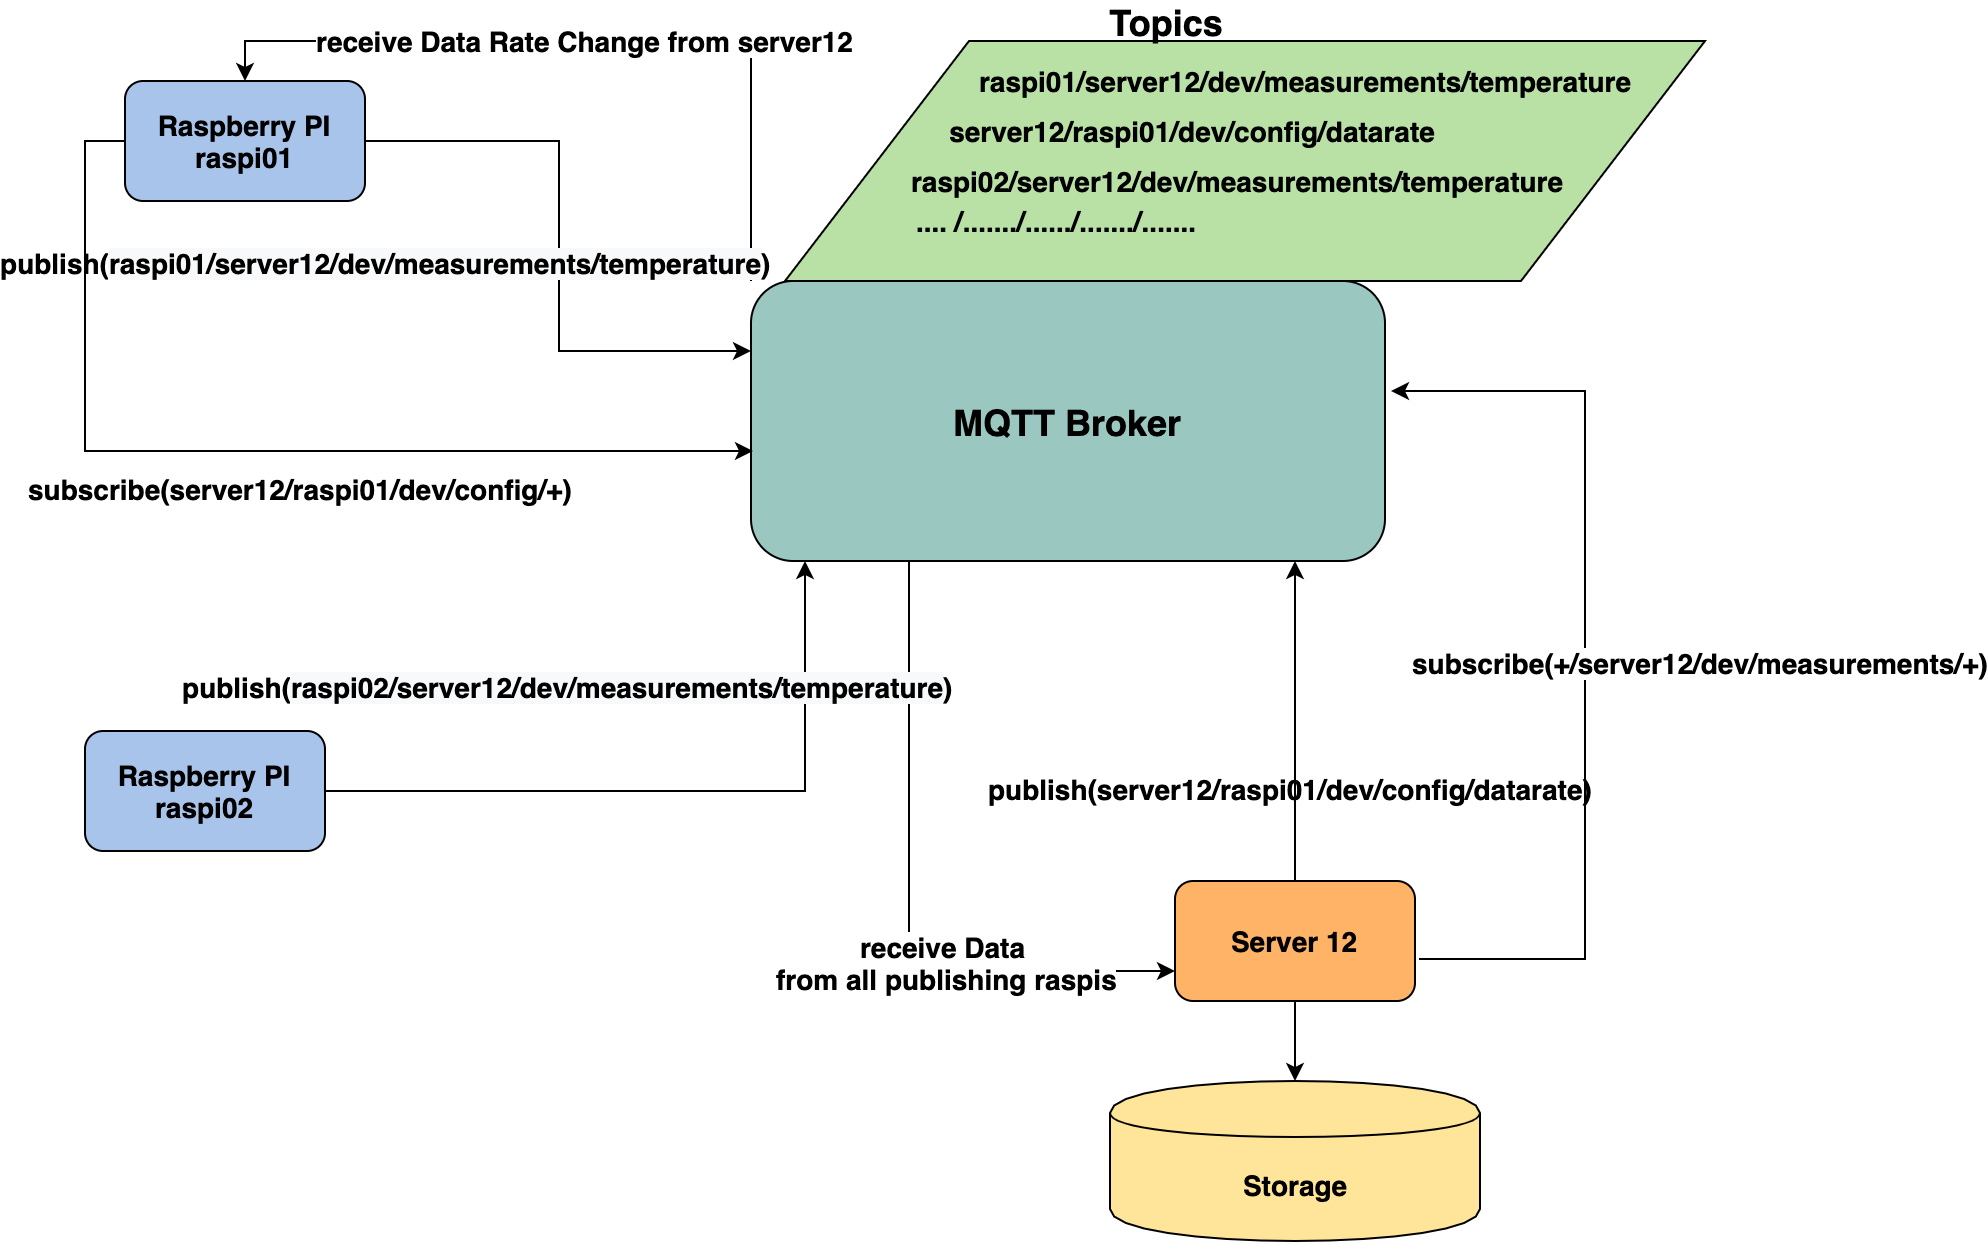
\includegraphics[scale=0.15]{7-datenaustausch/img/mqttarch} 
    \end{figure}
\end{frame}


%%% Folie
\begin{frame}{MQTT Topics}
     \begin{itemize}
        \setlength{\itemindent}{0.85in}
        \item [\textbf{MQTT Topics}]
    \end{itemize}
    \begin{itemize}
        \item Kommunikationskanal von einem oder mehreren Sender zu einem oder mehreren Empfängern
        \item Pfadartige hierarchische Struktur -  ähnlich zu Active Directory (Firma/Standort/Abteilung/Gebäude/...) oder File Explorer  (Laufwerk/Ordner/Unterordner/...) 
        \item Kann Wildcards enthalten:  \texttt{+} $\Rightarrow$ ersetze ein Pfadelement ,  \texttt{\#}  $\Rightarrow$ ersetze alle Pfadelemente ab der Position
        \item Empfohlene Topic Struktur:   Besitzer/Sender/Empfänger/Umgebung/Hauptthema/Unterthema/... , z.B.   \texttt{projektname/raspi01/server12/test/messdaten/lautstaerke}
        \item Umgekehrte Richtung:   \texttt{projektname/server12/raspi01/test/konfiguration/update}
        \item Hinweis: MQTT v5 sieht ein Antwort Topic vor
    \end{itemize}    
\end{frame}

%%% Folie
\begin{frame}{MQTT Protokoll - Quality Of Service: Definition}
   \begin{itemize}
        \setlength{\itemindent}{1.45in}
        \item [\textbf{Quality of Service (QoS}]
    \end{itemize}
    \begin{itemize}
        \item Parameter beim Datenversand, der sich auf Leistung (Traffic und Handling) sowie Zuverlässigkeit (Nachrichtenerhalt) auswirkt
        \item Muss für Publisher und Subscriber gewählt werden $\Rightarrow$ Bei der Planung darauf achten, dass je Use Case bei allen die QoS Level passen!
        \item QoS 0 $\Rightarrow$ Vielleicht ausliefern
        \item QoS 1 $\Rightarrow$ Einmal ausliefern oder auch mehrmals
        \item QoS 2 $\Rightarrow$ Genau einmal ausliefern
        \item Für QoS 1 und QoS 2 sind im Allgemeinen \textbf{Persistente Sessions} nötig, um den Zustand der Kommunikation stabil wiederherstellen zu können nach z.B. Reboot oder Downtime
    \end{itemize} 
\end{frame}

%%% Folie
\begin{frame}{MQTT Protokoll - Quality Of Service: Nachrichten}
   \vspace*{-1.5mm}
   \begin{figure}[!htb]
       \hspace*{5mm}
        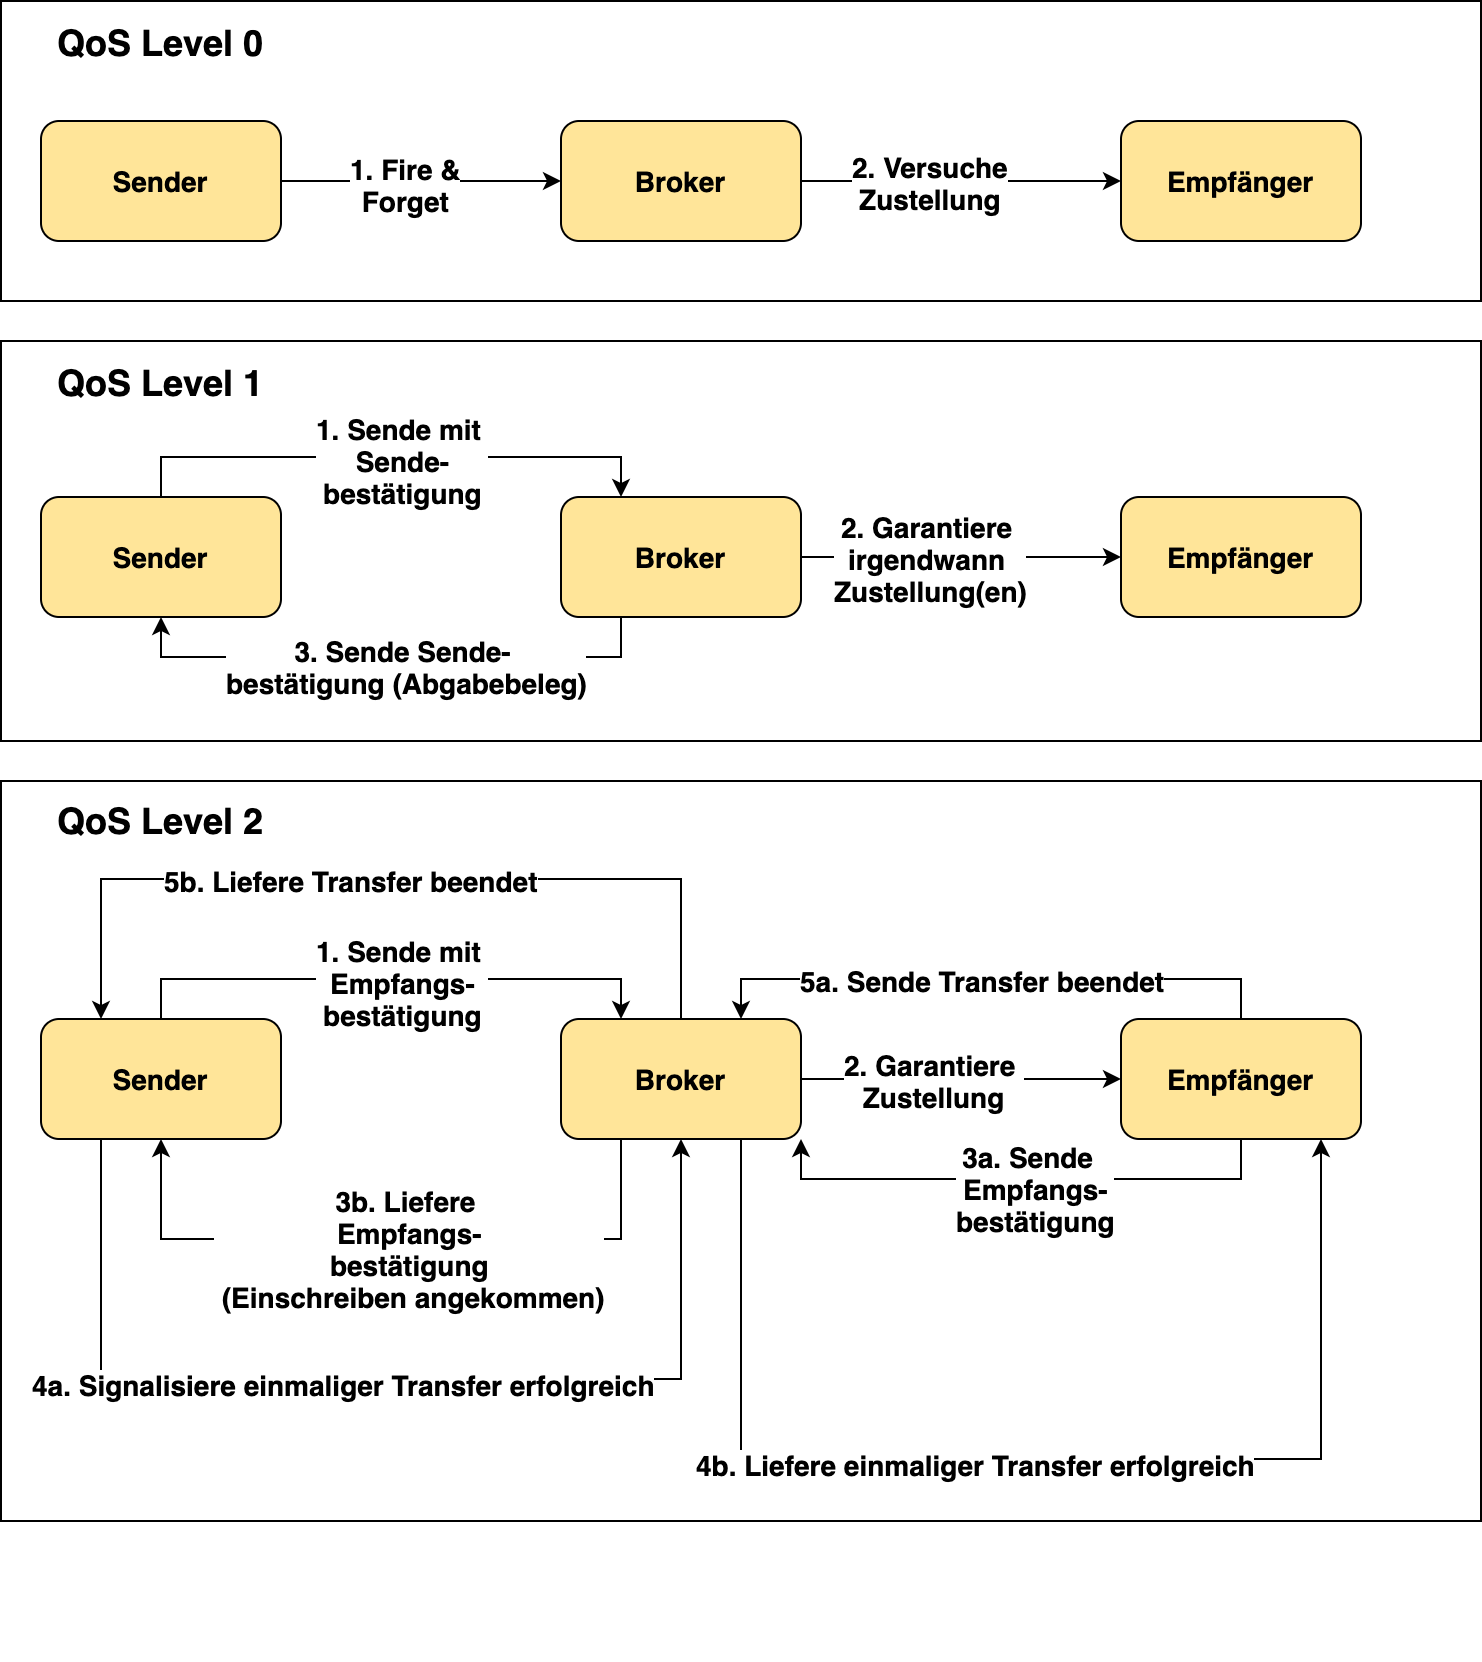
\includegraphics[scale=0.14]{7-datenaustausch/img/mqtt-qos} 
    \end{figure}
\end{frame}

%%% Folie
\begin{frame}{MQTT Protokoll: Retain Flag}   
      \begin{itemize}
        \setlength{\itemindent}{0.75in}
        \item [\textbf{Retain Flag}]
    \end{itemize}
    \begin{itemize}
        \item Flag für Nachrichten, damit diese am Topic erhalten bleiben $\Rightarrow$  spätere Subscriber bekommen diese als \quotes{Bootstrap Nachricht}, um sich über die letzte bekannte ordnungsgemäße Nachricht zu informieren
        \item Use Case: Status kontinuierlich überwachen
        \item Es gibt nur eine pro Topic
        \item Löschen über Nachricht mit leerem Content ohne Flag an das Topic
     \end{itemize} 
\end{frame}

%%% Folie
\begin{frame}{MQTT Protokoll: Last Will Testament}   
         \begin{itemize}
        \setlength{\itemindent}{1.2in}
        \item [\textbf{Last Will Testament}]
    \end{itemize}
    \begin{itemize}
        \item Nachricht, die beim Herstellen der Verbindung mitgegeben werden kann
         \item Wird an alle Subscriber des jeweiligen Topics gesendet
         \item Use Case: Client hat die Verbindung verloren und andere Clients müssen darauf reagieren können
    \end{itemize} 
\end{frame}


%%% Folie
\begin{frame}{MQTT Libraries}
              \begin{itemize}
        \setlength{\itemindent}{1.15in}
        \item [\textbf{Libraries für MQTT}]
    \end{itemize}
    \begin{itemize}
        \item Eclipse Paho für viele Programmiersprachen  $\Rightarrow$ \href{https://www.eclipse.org/paho/downloads.php}{eclipse.org/paho}
         \item Spring Integration MQTT Paho Wrapper für Java/Kotlin  $\Rightarrow$ \href{https://docs.spring.io/spring-integration/docs/5.2.1.RELEASE/reference/html/mqtt.html}{docs.spring.io}
         \item HiveMQ MQTT Client für Java  $\Rightarrow$ \href{https://www.hivemq.com/blog/mqtt-client-library-enyclopedia-hivemq-mqtt-client/}{hivemq.com}
         \item MQTT JS für NodeJS oder Browser $\Rightarrow$ \href{https://github.com/mqttjs/MQTT.js}{github.com/mqttjs/MQTT.js}
    \end{itemize} 
\end{frame}

%%% Folie
\begin{frame}{MQTT Broker}
          \begin{itemize}
        \setlength{\itemindent}{1.45in}
        \item [\textbf{Broker für die Architektur}]
    \end{itemize}
    \begin{itemize}
        \item Mosquitto  $\Rightarrow$ \href{https://mosquitto.org}{mosquitto.org}
         \item VerneMQ  $\Rightarrow$ \href{https://vernemq.com}{vernemq.com}
         \item HiveMQ Open Source  $\Rightarrow$ \href{https://www.hivemq.com/developers/community}{hivemq.com/developers/community}
    \end{itemize} 
\end{frame}


%-------------------------------------------------------------------------------
\section{Adafruit IO}
%-------------------------------------------------------------------------------

%%% Folie
\begin{frame}{Adafruit IO Einführung}
 \begin{itemize}
        \setlength{\itemindent}{1.4in}
        \item [\textbf{Adafruit IO Einführung}]
    \end{itemize}
    \begin{itemize}
        \item Cloud Backend zur einfachen Anbindung von IoT Devices wie Arduino, Raspberry PI
        \item Kann über MQTT Client und REST  API angesprochen werden  $\Rightarrow$ viele weitere Devices und Programmiersprachen werden somit unterstützt!
        \item Einfach konfigurierbare Dashboards mit verschiedenen Widgets
        \item \textbf{Trigger} Funktionen, um Aktionen in Drittsystemen auszulösen (E-mail senden etc.)
        \item Integration bestehender Cloud Services wie Wetterdaten oder If-This-Than-That
        \item Daten zwischen eigenen Projekten und Devices austauschen
    \end{itemize}    
\end{frame}


%%% Folie
\begin{frame}{Limits in der Freien Version}
  \begin{figure}[!htb]
  \hspace*{5mm}
        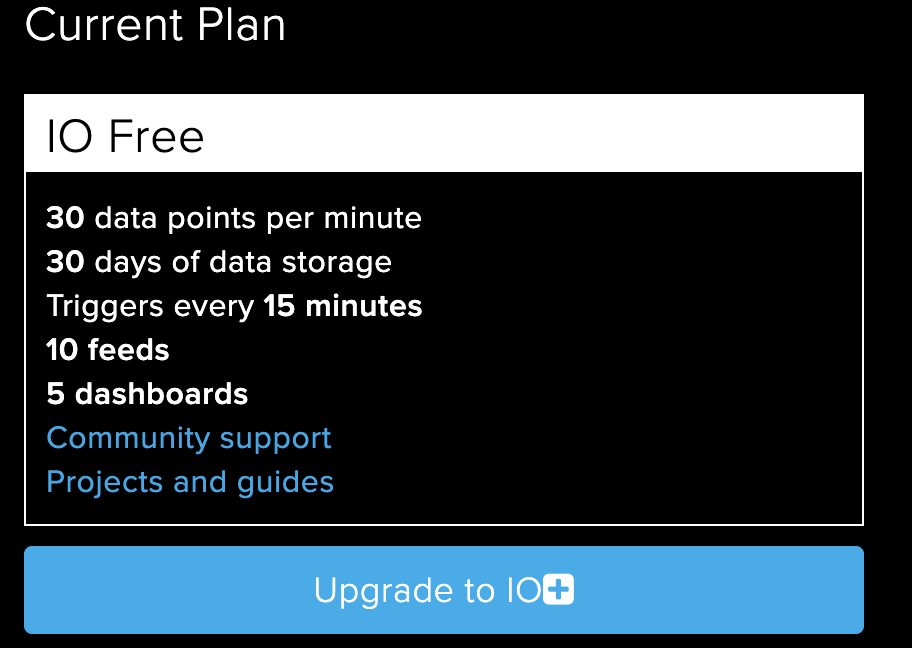
\includegraphics[scale=0.6]{7-datenaustausch/img/adafruit-limits} 
    \end{figure}
\end{frame}

%%% Folie
\begin{frame}{MQTT Client Integration}
        \begin{itemize}
        \setlength{\itemindent}{4.1in}
        \item [\textbf{Einrichtung eines Testclients (siehe auch:  \cite{Adafruit MQTTFx Setup}) }]
    \end{itemize}
      \vspace*{-5mm}

  \begin{figure}[!htb]
  \hspace*{2mm}
        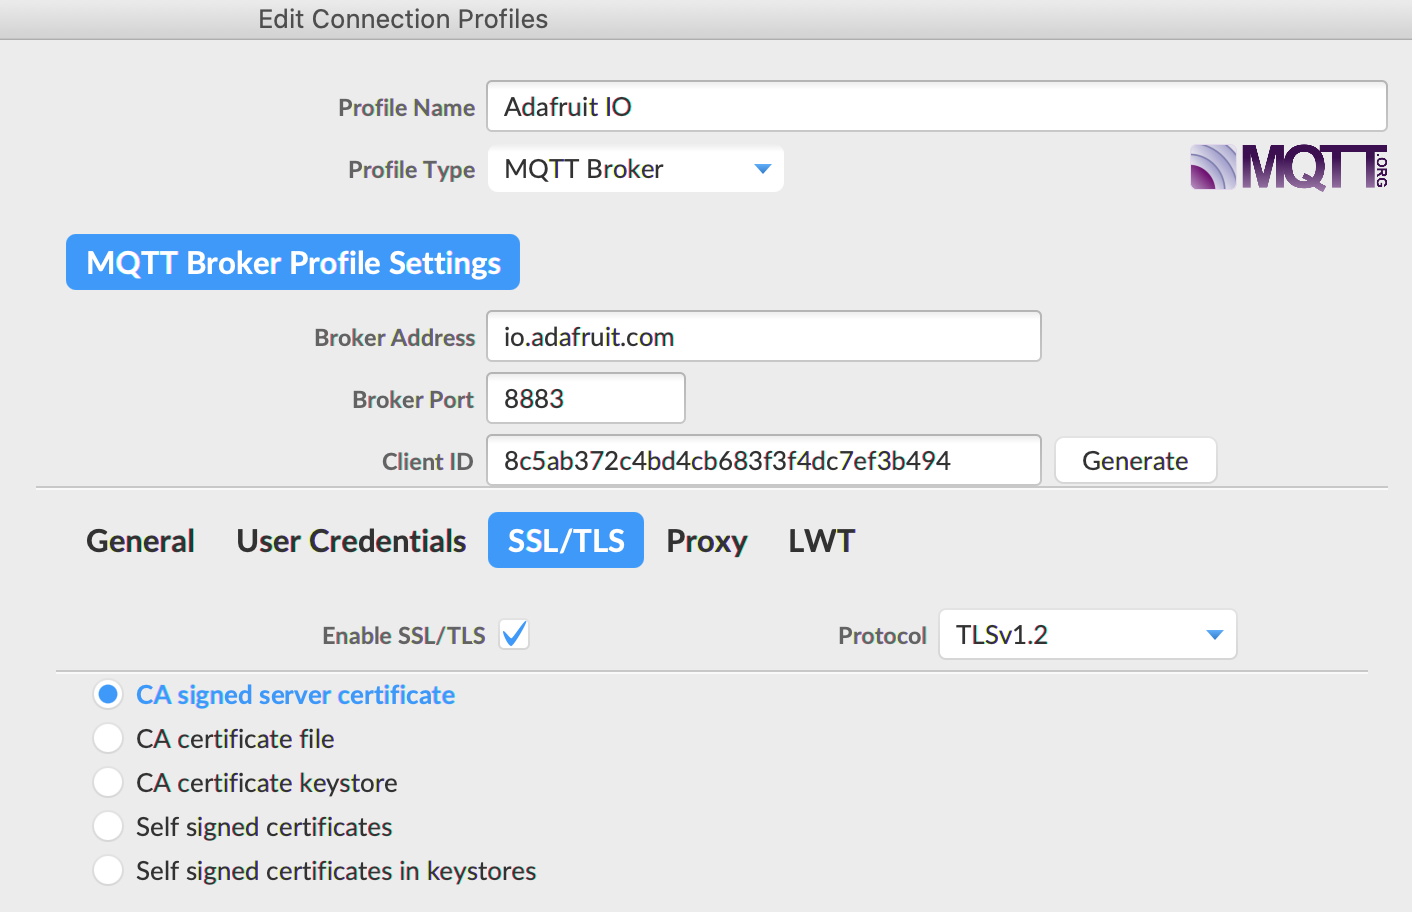
\includegraphics[scale=0.4]{7-datenaustausch/img/mqttfxsettings} 
    \end{figure}
\end{frame}

%%% Folie
\begin{frame}{MQTT-over-WebSocket im Browser}
      \vspace*{-1.5mm}
    \begin{figure}
	\centering
	\parbox{5cm}{
		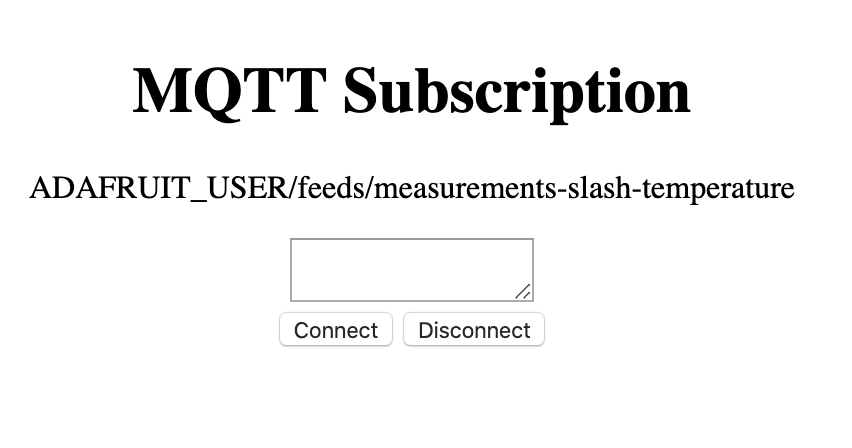
\includegraphics[scale=0.19]{7-datenaustausch/img/websocket-mqtt-min}
		\caption{MQTT-over-Websockets Topic Subscription}
		\label{fig:wsmqttmin}
		}
	\qquad
	\begin{minipage}{5cm}
		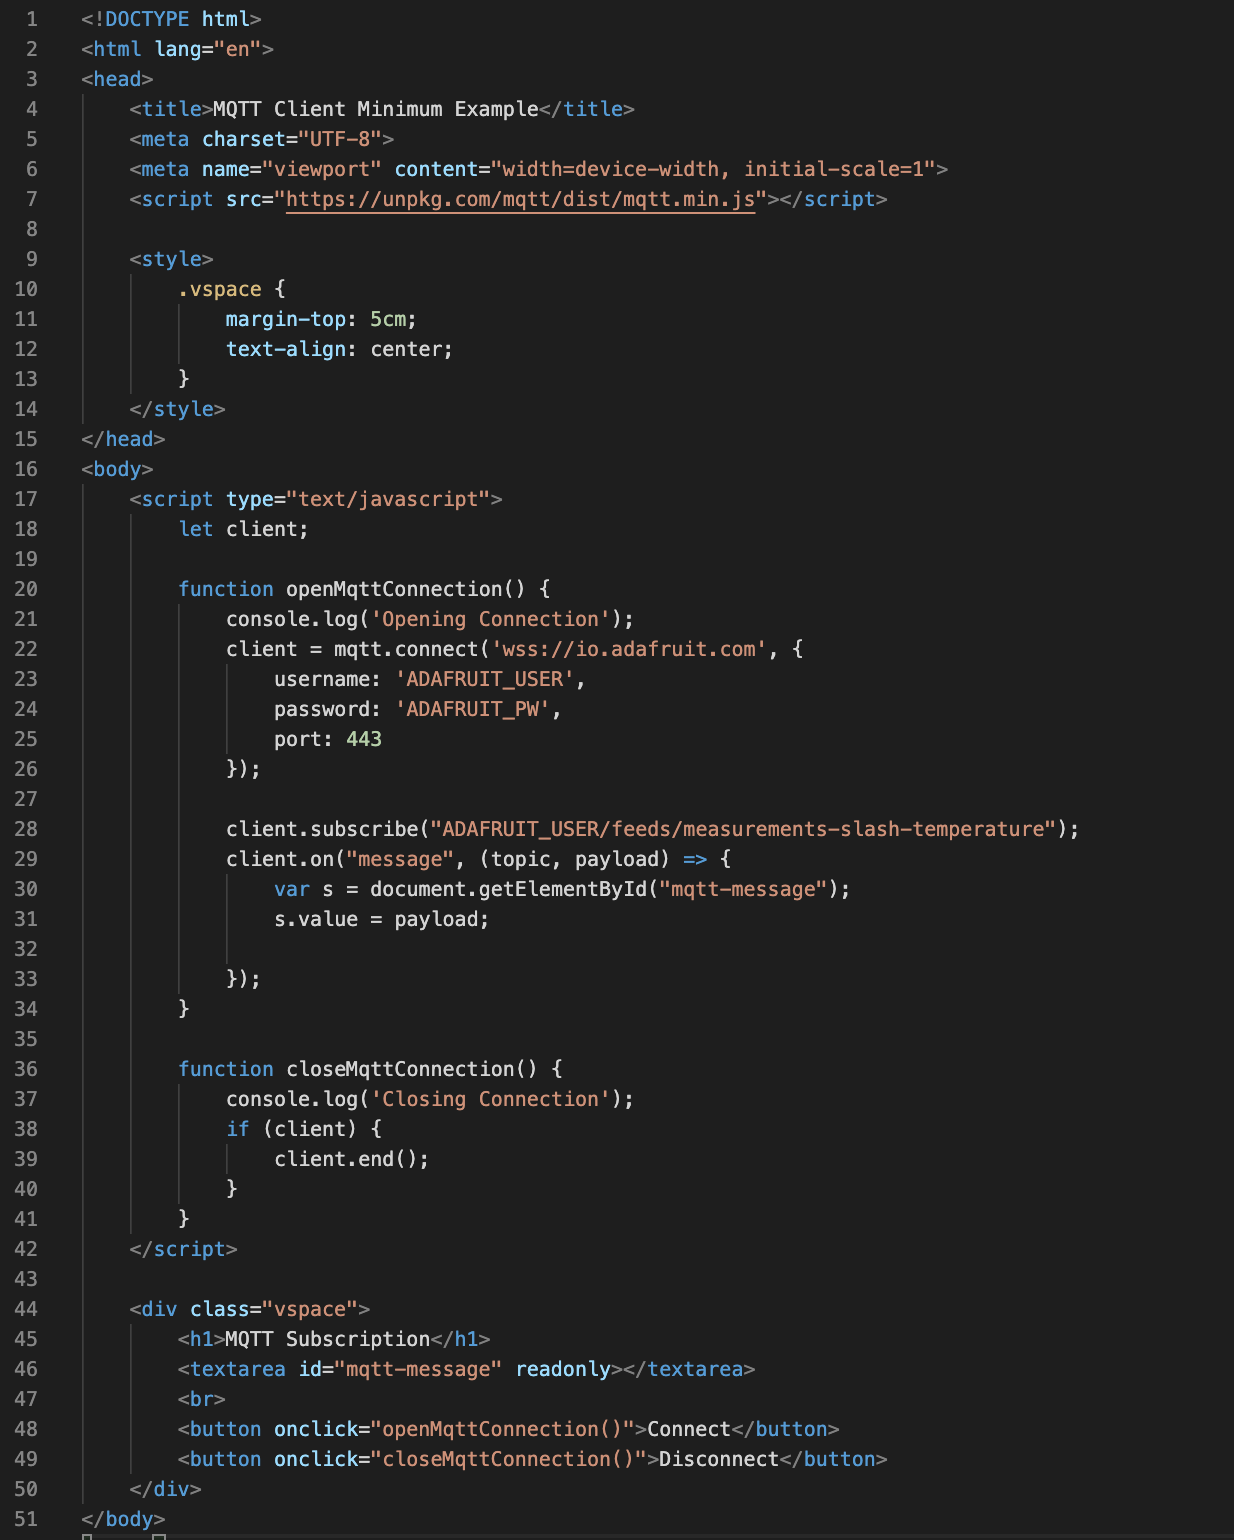
\includegraphics[scale=0.27]{7-datenaustausch/img/websocket-mqtt}
		\caption{JS und HTML Code}
		\label{fig:wsmqtt}
	\end{minipage}
	\end{figure}

\end{frame}


%%% Folie
\begin{frame}{Unterschiede im Topic Handling}
    \begin{itemize}
        \setlength{\itemindent}{1.6in}
        \item [\textbf{Adafruit IO Besonderheiten}]
    \end{itemize}
    \begin{itemize}
        \item Statt der Topic Struktur aus MQTT werden im Adafruit IO sogenannte  \textbf{Feeds} verwendet \cite{io.adafruit.com/api/docs}
        \item Feeds sind \quotes{mehr als nur Topics}: Metadaten, Nachrichten, Lizenzinformation, Sichbarkeitskontrolle (private vs. public)
        \item Feeds können auch per REST API bedient werden:  \texttt{POST/api/v2/{username}/feeds} mit Inhalt z.B. Name/Beschreibung des Feeds
        \item In Adafruit gestalten sich Topics nach folgender Semantik: \texttt{userName/feeds/groupName.feedkey} \cite{Adafruit und MQTT Topics}
        \item Achtung: \underline{weitere} Slashes in Namen von Topics werden automatisch ersetzt durch \texttt{-slash-}
    \end{itemize}    
\end{frame}

%%% Folie
\begin{frame}{Unterschiede bei Pub/Sub}
	\begin{figure}
	\centering
	\parbox{5cm}{
		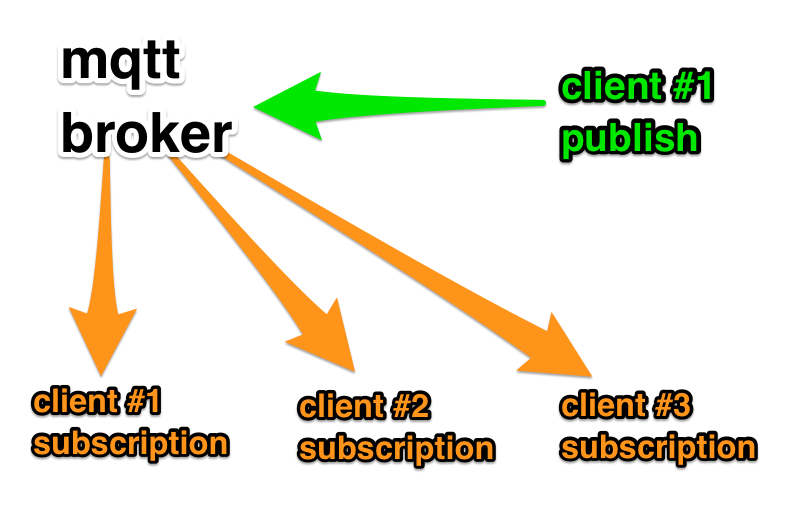
\includegraphics[scale=0.19]{7-datenaustausch/img/mqtt-pubsub}
		\caption{Pub/Sub in MQTT}
		\label{fig:pubsubmqtt}
		}
	\qquad
	\begin{minipage}{5cm}
		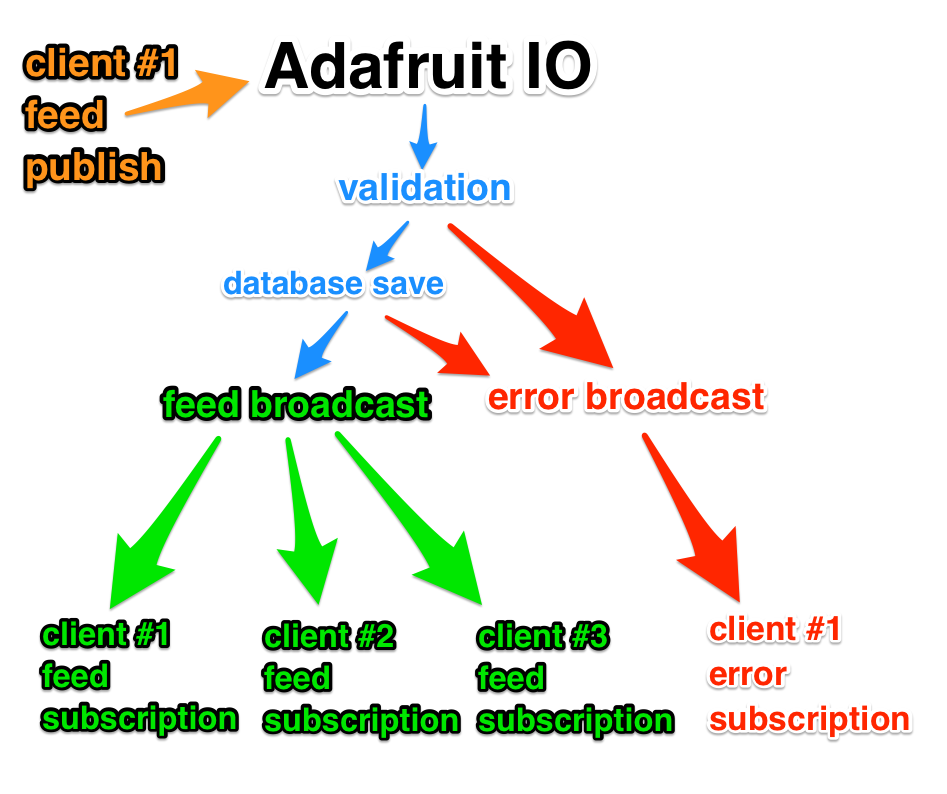
\includegraphics[scale=0.15]{7-datenaustausch/img/adafruit-pubsub}
		\caption{Pub/Sub in Adafruit}
		\label{fig:pubsubadafruit}
	\end{minipage}
	\end{figure}
\end{frame}

%%% Folie
\begin{frame}{Adafruit IO: Python Code Beispiel}
    \begin{figure}
       \hspace*{2mm}
        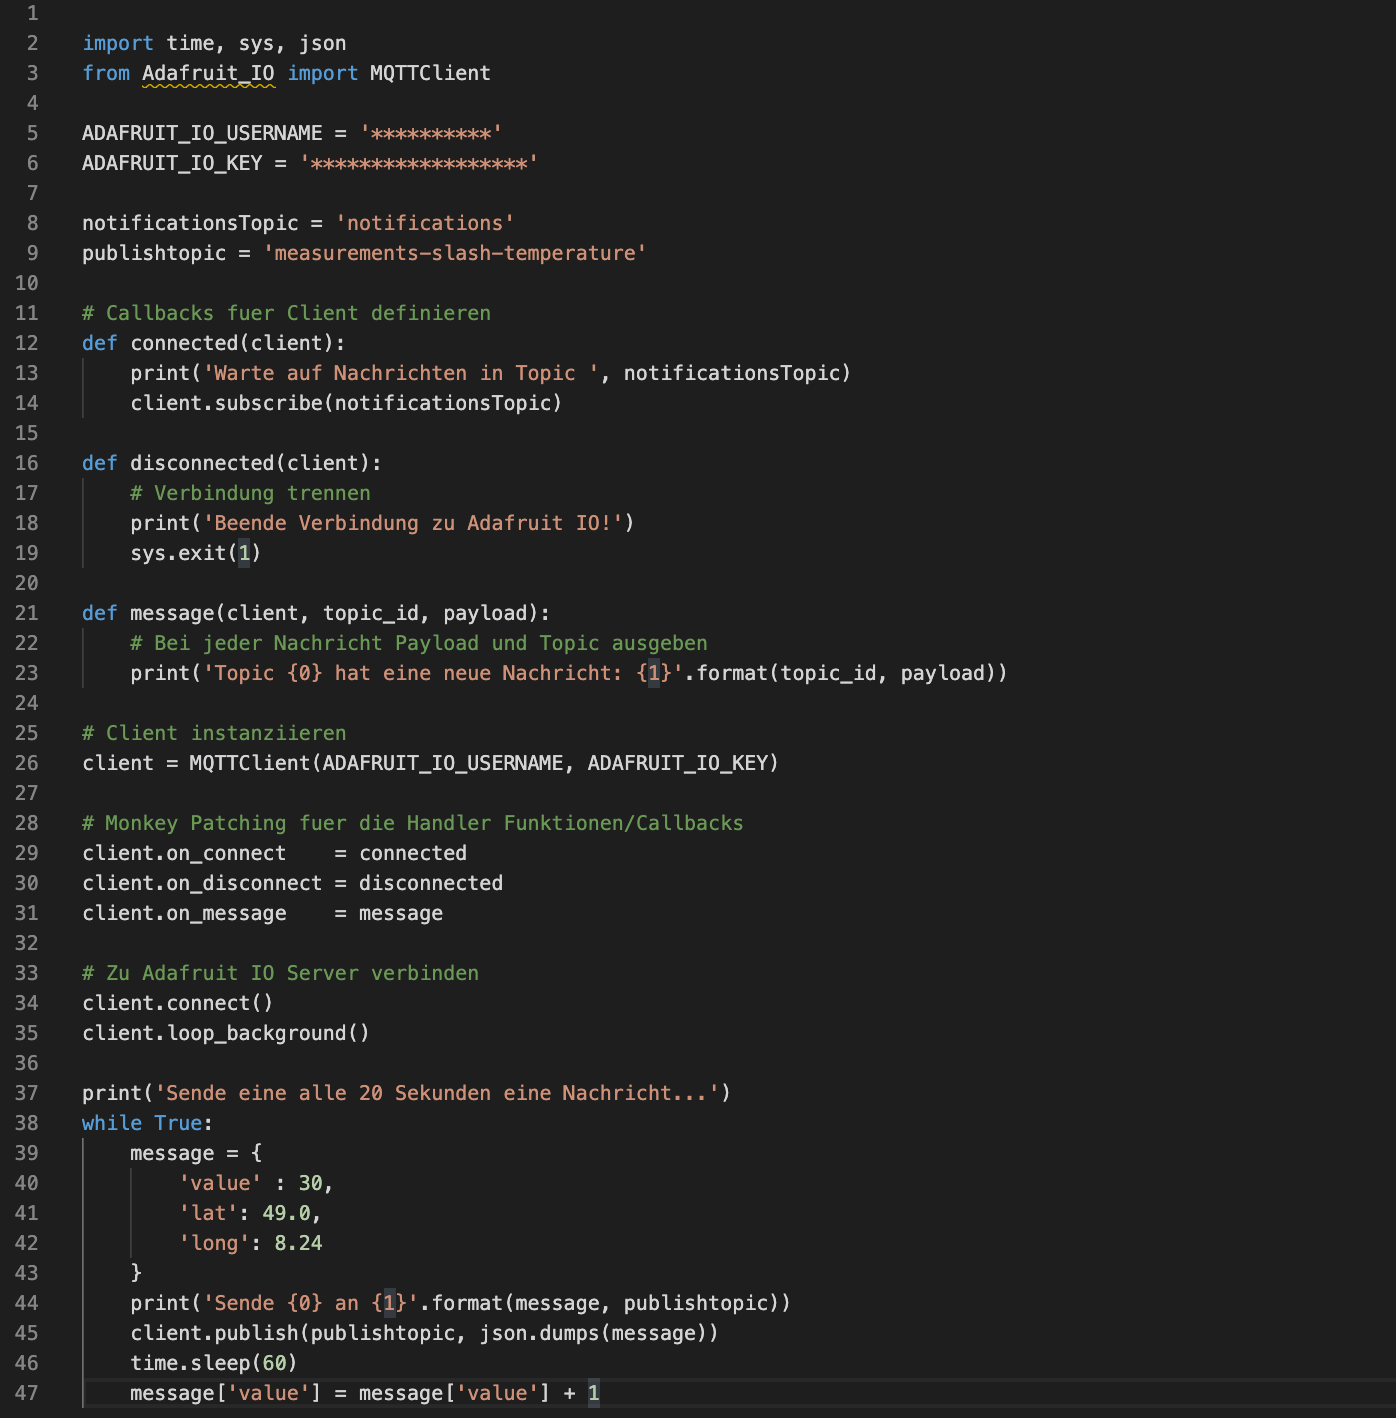
\includegraphics[scale=0.28]{7-datenaustausch/img/adafruit-python-mqtt} 
    \end{figure}
 \end{frame}


%%% Folie
\begin{frame}{Adafruit IO Dashboard: Live DEMO}
      \centering
  	\begin{Huge}
      		\textbf{LIVE DEMO}
	\end{Huge}
\end{frame}



